\documentclass[DM,authoryear,toc]{lsstdoc}
\newcommand{\czw}[1]{
  \textbf{CZW: }\textcolor{red}{#1}
}

% lsstdoc documentation: https://lsst-texmf.lsst.io/lsstdoc.html
\input{meta}

% Package imports go here.

% Local commands go here.

%If you want glossaries
%\input{aglossary.tex}
%\makeglossaries

\title{Calibration Generation, Verification, Acceptance, and Certification.}

% Optional subtitle
% \setDocSubtitle{A subtitle}

\author{%
Chris Waters
}

\setDocRef{DMTN-222}
\setDocUpstreamLocation{\url{https://github.com/lsst-dm/dmtn-222}}

\date{\vcsDate}

% Optional: name of the document's curator
% \setDocCurator{The Curator of this Document}

\setDocAbstract{%
This technote defines the best practices to be used for calibration generation, the verification that that calibration meets requirements, and when deciding if the calibration should be accepted for use in processing at both the summit and USDF.
}

% Change history defined here.
% Order: oldest first.
% Fields: VERSION, DATE, DESCRIPTION, OWNER NAME.
% See LPM-51 for version number policy.
\setDocChangeRecord{%
  \addtohist{1}{2022-03-21}{Initial draft.}{Chris Waters}
  \addtohist{2}{2022-09-16}{Corrected and clarified draft.}{Chris Waters}
  \addtohist{3}{2024-04-17}{Updated draft reflecting processes actually in use.}{Chris Waters}
  \addtohist{4}{2024-11-08}{Updated draft with further details on processes}{Chris Waters}
}


\begin{document}

% Create the title page.
\maketitle
% Frequently for a technote we do not want a title page  uncomment this to remove the title page and changelog.
% use \mkshorttitle to remove the extra pages

% ADD CONTENT HERE
% You can also use the \input command to include several content files.

\section{Introduction}

The purpose of this technote is to provide guidance on the procedures that are used for the construction and management of calibrations.
These guidelines shall be followed for any calibration that will be added to the main butler repositories.  For the purposes of this document, we will consider three cases of calibrations.

\begin{itemize}
\item Calibrations generated for widespread use, using the main butler repository.  These are referred to as ``combined calibrations'' below, and indicate the calibrations that are used for science processing.
\item Curated calibrations that are defined by an \verb|obs_| package and must be ingested to the butler repository, as they cannot be directly generated from raw data.  The camera geometry calibration is an example of this type of calibration.
\item Calibrations that have been exported from one butler repository for use in another.
\end{itemize}

Additional private calibrations produced for tests may also exist, but as those will only exist in a user-space collections, they will not be discussed further in this document.

Briefly, calibration construction involves the following steps:
\begin{description}
\item[Generation] An appropriate set of exposures is chosen and processed through the correct \verb|cp_pipe| pipeline.
\item[Verification] The proposed calibration is used to process exposures through the matching \verb|cp_verify| pipeline.  This processing measures a set of quality metrics, as defined by DMTN-101, to determine if the newly made calibration meets requirements.
\item[Certification] The proposed calibration is certified for a particular usage date range.  These are generally open ended, with only the start date defined.  We expect to know the start date for the majority of all calibrations, as they should correspond with changes to the camera.
\item[Approval] The TAXICAB considers the proposed calibrations and their associated verification results, and makes the decision on whether the proposal is accepted for use.
\item[Distribution] The collection containing the new calibrations are included in the main calibration collection chain, for all repositories that need the updated calibration.
\end{description}

Figure \ref{fig:flowchart} displays the relationship between the various stages of construction, validation, and use of combined calibrations. \czw{Is this still useful?}

\begin{figure}
  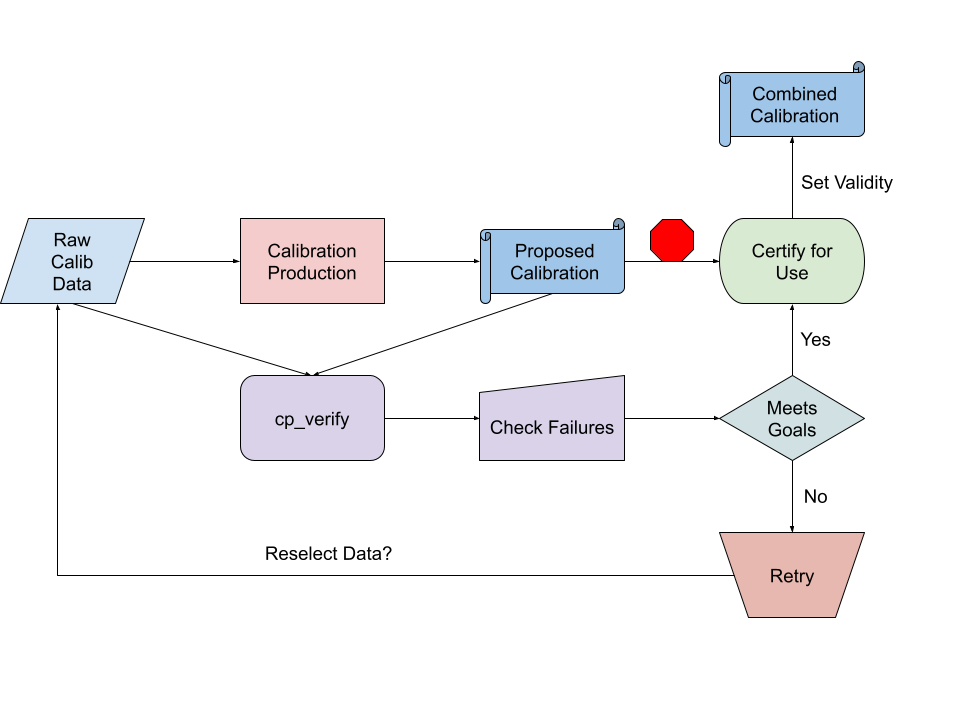
\includegraphics[width=\linewidth]{figures/flowchart.png}
  \caption{Flowchart of the calibration construction process.}
  \label{fig:flowchart}
\end{figure}

\section{Collection naming}

Consistent collection names make the management of calibrations easier.
JIRA tickets are used to ensure that these collection names are unique, and that there is a clear location to find the construction artifacts for later analysis.
In addition to this ticket, a short string explaining the purpose of the calibration set should be included in the collection name to provide a human readable ``tag.''
The following collection name patterns, based on the recommendations in DMTN-167 should be followed for all calibrations that will be approved by the TAXICAB.

The calibration generation should use the form
\begin{verbatim}
  $INSTRUMENT/calib/$TICKET/$TAG/${CALIB_TYPE}Gen.${RERUN_ITERATION}
\end{verbatim}
where \verb|$INSTRUMENT| is the camera name, \verb|$TICKET| is the JIRA ticket value, \verb|$TAG| is the short human readable string, \verb|$CALIB_TYPE| is the calibration type being generated, and \verb|$RERUN_ITERATION| is a date string of the form \verb|YYYYMMDDv| indicating when the calibration was made, with a trailing character to be incremented if the generation must be retried.
As an example, a hypothetical new bias would have a collection name like \verb|LATISS/calib/DM-12345/voltageChange/biasGen.20220915a|.

For verification, a similar form is used:
\begin{verbatim}
  $INSTRUMENT/calib/$TICKET/$TAG/verify${CALIB_TYPE}.${RERUN_ITERATION}
\end{verbatim}
with the same elements as for generation.
The certification process (see below) also creates a new CALIBRATION collection, which should just contain the calibration type:
\begin{verbatim}
  $INSTRUMENT/calib/$TICKET/$TAG/${CALIB_TYPE}.${CERTIFICATION_RERUN}
\end{verbatim}
These CALIBRATION collections should be added to a CHAINED collection that uses the collection base only up to the ticket.
This ticket-level CHAINED collection provides a way to add and remove all of the calibrations constructed as part of that ticket in one operation.
In addition, by ensuring that new calibration collections are prepended to the top level CHAINED collection, we can avoid needing to set end dates during calibration certification.
The butler search for calibrations completes when the first matching calibration is found.
So, as an example, by putting a collection with a start date of 2024-10-01 before one with a start date of 2024-06-01, we can ensure that an exposure taken on 2024-10-15 will be processed with that newer calibration, but one taken on 2024-09-01 will be processed with the older one.

\section{New Combined Calibrations Construction}

A record of the calibration construction process should be retained and attached to the JIRA ticket managing the work, with all commands executed and exposure selections recorded.
Having this record will allow for understanding what happened during construction, in case the final products have problems.

\subsection{Generation}

Combined calibrations will be generated directly from raw exposures as much as possible.
The tasks and pipelines in the \verb|cp_pipe| package can produce all of the calibrations that are currently used for image processing, and can be supplemented as new corrections are developed.
The main documentation for calibration construction is included in \verb|cp_pipe| at \url{https://pipelines.lsst.io/v/daily/modules/lsst.cp.pipe/constructing-calibrations.html}, but the main points will be summarized here.

Calibrations are inter-dependent, and so the construction of one type may require precursor calibrations to be built first.
Figure \ref{fig:dependence} shows the current dependence, with each box pointing to the calibrations that they depend on.
The result of this is that changes in one calibration (such as the gains derived from the photon transfer curve) require other calibrations (the linearity, the brighter-fatter kernel, and the charge transfer inefficiency) to be built as well.

\begin{figure}
  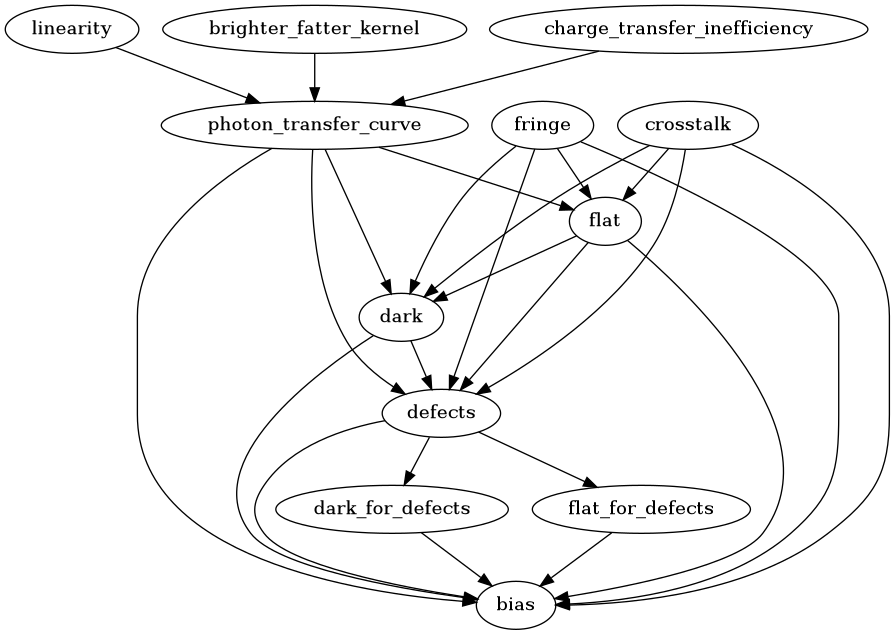
\includegraphics[width=\linewidth]{figures/dependence.png}
  \caption{Dependency charge of calibration products.  The arrow indicates the parent calibration.}
  \label{fig:dependence}
\end{figure}

The \verb|observation_type| and \verb|observation_reason| of the input exposures should match the calibration type to be constructed, with the exception of the fringe and crosstalk calibrations, which are constructed from science exposures.
Most calibrations can be constructed from a single set of daily calibrations, with the number of bias, dark, and flat frames in these sets (generally of order 15-20) sufficient to create a usable combined calibration.
Dense PTC curves will require many more inputs (on the order of 100 pairs of exposures), and we currently expect that we will have dedicated observation sequences for this purpose.

Calibrations constructed for general use should be able to use the version of the \verb|cp_pipe| tasks and pipelines on the main github branch.
It is preferable to keep code development separate from the calibration construction, but it is expected that these will likely be coupled during commissioning.

To ensure all butler repositories have a consistent set of calibrations, we have decided that only one processing location should perform the calibraion construction steps.
The US Data Facility (USDF) is now operational, all calibrations used for the survey will be generated there.
The process for transferring the calibrations to other butler sites is discussed below in Section \ref{sec:calib_export}.

\subsection{Verification}
A verification report is then generated from the generation and verification collections, and will be supplied to the Telescope And auXiliary Instrumentation Calibration Acceptance Board (TAXICAB).

Once the proposed calibrations have been generated, the calibration should be used for processing using the \verb|cp_verify| tasks and pipelines.
These tasks measure quality metrics from those processed exposures, and identify any test failures.
At a minimum, the exposures used to construct the calibration should be included, as this can identify problematic inputs that degrade the calibration quality.
An example of this is saturated flat exposures, which do not flat-field well, and should not be included in the final flat calibration.
In running the \verb|cp_verify| tasks, the input butler collections specified should have the construction RUN collection placed at the beginning of the list, to ensure that the verification process will find and use the calibration we wish to verify.

Exposures from outside the set used for construction should be added to provide insight into the expected validity range for the calibration.
As long as the metrics on those exposures remain within the limits defined in DMTN-101, the calibration may continue to be valid for the date range including those additional exposures.
This can be used to establish the valid date ranges to be used when certifying the calibration.

The \verb|cp_verify| pipelines will generate and publish \verb|analysis_tools| ``core'' metrics and plots to cover the DMTN-101 tests.
These metrics and plots will also include useful diagnostic results based on the camera team \verb|eo_pipe| tests.
Further ``extended'' metrics and plots may also need to be generated to supply additional debugging information about the calibrations.

The \verb|cp_verify| report is generated by a command such as
\begin{verbatim}
$CP_VERIFY_DIR/bin/cpv_report.py -r /repo/embargo \
                    -O ~/public_html/cpv_reports/TAXICAB-15 \
                    -c LSSTComCam/calib/DM-47447/gainFixup/verifyFlat-g.20241107a \
                    -c LSSTComCam/calib/DM-47447/gainFixup/verifyFlat-r.20241107a \
                    -c LSSTComCam/calib/DM-47447/gainFixup/verifyFlat-i.20241107a \
                    -c LSSTComCam/calib/DM-47447/gainFixup/verifyBias.20241107a \
                    -c LSSTComCam/calib/DM-47447/gainFixup/verifyDark.20241107a \
                    -c LSSTComCam/calib/DM-47447/gainFixup/flatGen-g.20241107a \
                    -c LSSTComCam/calib/DM-47447/gainFixup/flatGen-i.20241107a \
                    -c LSSTComCam/calib/DM-47447/gainFixup/flatGen-r.20241107a \
                    -c LSSTComCam/calib/DM-47447/gainFixup/darkGen.20241107a \
                    -c LSSTComCam/calib/DM-47447/gainFixup/atoolsDark.20241108a \
                    -c LSSTComCam/calib/DM-47447/gainFixup/atoolsDarkDet.20241108a
\end{verbatim}
As many collections and types of calibrations can be added to the list of inputs.
All applicable verify collections should be included, and although the generation collections should be linked from the verify collection (allowing them to be searched for data products), it is generally safe to add them to the list as well.
This report constructs set of HTML documents and web-friendly images so the calibration quality can be checked.
The report is known to be incomplete, as there is a large backlog of tickets for adding plots and metrics to the code.

\subsection{Certification}

Once the new combined calibration has been generated and verified, it can be certified for use for a given date range.
Calibrations that have been constructed due to a camera or telescope change, or that are being built to replace another calibration that is no longer within the test specifications, should always have a starting validity date, with the end date left open.
This ensures that future data taken will always have valid calibrations for processing.

If historical calibrations are being constructed, the end date should be known from the daily calibration processing results stored in the visit database (see below).
Future development is needed to allow calibrations to be recertified to update the date ranges.

The certification process can be done with a simple butler command:
\begin{verbatim}
butler certify-calibrations $REPO \
    --begin-date $START_DATE \
    $INSTRUMENT/calib/$TICKET/$TAG/biasGen.$RERUN \
    $INSTRUMENT/calib/$TICKET/$TAG/bias.${CERT_RERUN} \
    bias
\end{verbatim}
where the \verb|$START_DATE| is the ISO-8601 datetime in TAI coordinates, and \verb|$CERT_RERUN| is a dated rerun string as used above (as the generation and certification may take place on different dates).

Note that certification is purely a ``database operation,'' with the certified collection gaining a ``link'' to the dataset in the construction collection.
This means that if the underlying generation collection is removed, the calibrations may be lost as well.

\subsection{Approval}

With the calibrations built, verified, and certified, a TAXICAB ``hailing'' ticket should be created, with a verification report attached for consideration.
Any member of the Rubin Observatory Team is welcome to join the TAXICAB meeting, and the meeting will make decisions as a consensus.
Any additional processing that is suggested by the TAXICAB should be defined and run prior to the TAXICAB meeting, which will have a planned weekly timeslot.
Currently, this meeting is scheduled for Tuesday at 2pm Project Time.
If no open TAXICAB hailing tickets exist, this meeting will be skipped.
Scheduling a TAXICAB meeting generally indicates that the associated ticket has been marked as ``Flagged,'' as it is awaiting the decision on acceptance.

The TAXICAB will consider the verification reports, identify any potential issues with the calibration set, and determine if any verification test failures warrant restarting the construction process to address the issues.
Ideally, all verification metrics will succeed, and a quick check of residual exposures will show no unexpected features.
In the more likely case that some fraction of these tests fail, the TAXICAB will be tasked with deciding if the failures are fatal and that the calibration should be fully rejected, or if the failures are small enough in number or impact that the calibration can be accepted for use despite them.
The TAXICAB will operate on a consensus basis, to ensure that all stakeholders have input on this process.

If the calibrations were built using a ticket/development branch of any software, those code changes must be reviewed and approved through the standard DM process prior to hailing the TAXICAB.
If no new code was added, then the approval of the TAXICAB can be used as the review process to close the initial generation ticket.

Managing the approval for calibrations will follow a three-ticket process.
As described above, a construction ticket is used to manage all construction, verification, and certification steps, and is included in all output collection names.
A TAXICAB ticket is used to manage the approval of the calibrations, and to contain pointers to the verification report, the generation ticket, and the final ticket, which manages the deployment of these calibrations.
This deployment ticket is used for copying the calibration into all necessary public repositories, as described below.
If code was added as part of the construction, that work should be reviewed on the construction ticket prior to the TAXICAB meeting.
Otherwise, the TAXICAB approval (by marking that ticket ``Adopted'') should also mark the construction ticket as reviewed.
The deployment ticket will be self-reviewing in the future: a trivial processing task should be run at each repository that has had the new calibrations deployed, with checks that those new calibrations are correctly selected and used.

\subsection{Distribution}
\label{sec:calib_export}
Upon approval of the TAXICAB, the calibrations can be distributed for use.
A separate distribution ticket should be created to handle this work, and linked to both the construction ticket and the TAXICAB ticket.
As the calibrations have already been certified in the origin butler repository, the distribution process for that repository simply needs a CHAINED collection added that contains all of the calibrations generated on the construction ticket.
In most circumstances in which new forward-looking calibrations are deployed, this new CHAINED collection can be prepended to the top level calibration CHAINED collection, installing the calibration for use.

The calibrations must then be exported for use in other repositories, with the butler repository at the summit being most important to update.  An example command to do such is
\begin{verbatim}
butler export-calibs $REPO ./export_directory LATISS/calib/DM-XYZ LATISS/calib/DM-XYZ/voltageChange/bias [...]
\end{verbatim}
This command exports the files into the \verb|export_directory| location, and constructs a YAML description of the calibrations and their collections.
Exporting the ticket-level CHAINED collection will export all of the children CALIBRATION collections, making it the preferred way to export calibrations.
It is strongly recommended that the file permissions are checked in the \verb|export_directory| to ensure that the files are world readable.
The import process will create files with the same permissions, so this check is essential to prevent processing problems.

This \verb|export_directory| must then be transferred to the location of the new repository, where it can be imported with the command
\begin{verbatim}
butler import $NEW_REPO  --transfer copy \
       --export-file ./export_directory/export.yaml ./export_directory \
       -s instrument -s detector -s physical_filter
\end{verbatim}

The \verb|--transfer copy| is strongly suggested, as this will copy the files into the repository datastore, removing any dependency on the \verb|export_directory|.
The three \verb|-s| arguments indicate that the \verb|instrument|, \verb|detector|, and \verb|physical_filter| definitions contained the the YAML description should be skipped, as they will already exist in a repository that has been set up for the appropriate camera.

The newly imported collections will not by default be part of the main public calibration collection.
To do so, the new collections must be added to the collection chain.
Using the following command with the `prepend` mode will add the new collections to the start of the collection chain, making them available.
\begin{verbatim}
butler collection-chain $NEW_REPO --mode=prepend LATISS/calib \
       LATISS/calib/DM-XYZ \
       LATISS/calib/DM-ABC
\end{verbatim}
The distribution ticket should be able to be self-reviewed, after confirming that at least one exposure from the validity range of the new calibrations can be processed through \verb|IsrTask|, and that the output processed exposure has the correct calibration information recorded in its header.

The following table lists the current set of facilities, repositories, and which cameras are deployed in that repository.
\begin{tabular}{lll}
  Data Facility & Repository & Camera \\
  \hline
  USDF & embargo\_old & LATISS \\
  & & LSSTComCam \\
  & & LSSTComCamSim \\
  & & LSSTCam \\
  \hline
  USDF & /repo/embargo & LATISS \\
  & & LSSTComCam \\
  & & LSSTComCamSim \\
  & & LSSTCam \\
  \hline
  USDF & /repo/main & LATISS \\
  & & LSSTComCam \\
  & & LSSTComCamSim \\
  & & LSSTCam \\
  \hline
  USDF & /repo/ir2 & LSSTCam \\
  \hline
  Summit & /repo/LATISS & LATISS \\
  Summit & /repo/LSSTComCam & LSSTComCam \\
  & & LSSTComCamSim \\
  Summit & /repo/LSSTCam & LSSTCam \\
  \hline
  Tucson Test Stand (TTS) & /repo/LATISS & LATISS \\
  Tucson Test Stand (TTS) & /repo/LSSTComCam & LSSTComCam \\
  & & LSSTComCamSim \\
  \hline
\end{tabular}

\subsubsection{Summit Cleanup}

Files in the butler repos at the summit and TTS are subject to an automated cleaning process.
We can avoid having calibrations cleaned by ensuring that they are added to TAGGED collections.
These collections mark the datasets as important, preventing the automated cleaning from removing them.
After ingesting and chaining the newly imported calibrations, a series of \verb|butler associate| commands should be run to create the TAGGED collections.
These TAGGED collections do not have validity date ranges associated with them, and so care must be taken that two datasets with the same dataId are not associated into the same TAGGED collection.
An example association command is
\begin{verbatim}
butler associate $REPO \
       LSSTComCam/calib_tagged/DM-46360 \
       -d bias \
       --collections LSSTComCam/calib/DM-46360/isrTaskLSST/biasGen.20240926a/20240927T212215Z
\end{verbatim}
which must manually iterate over all calibration dataset\_type/generation collection pairs.
This TAGGED collection should never be used for processing, and is simply an accounting step to prevent cleanup.
Keeping these collections prefixed with \verb|$INSTRUMENT/calib_tagged/$TICKET| makes it clear that they're not intended for processing, but allows calibrations generated at the same time to be grouped together.

\subsection{Auxilliary Data Products}

In addition to calibrations that are directly used in the processing of data, there are other data products that are managed and distributed by the calibrations team to ensure that repositories are consistent.
These datasets are generally added to the \verb|$INSTRUMENT/defaults| CHAINED collection, which links the raw exposure collection, the top level CHAINED calibration collection, and other standard data products that are needed for completely processing.
The two most common of these data products are reference catalogs (refcats) and skymaps.

\subsubsection{Refcats}

\czw{This needs to be written.}

\subsubsection{Skymaps}

The skymaps contain the spatial information about the tracts and patches used for coadd construction.
The standard skymap configuration files can be found in \czw{a TBD archive}.
The information about these skymaps is stored in the butler database, and not as standard on-disk files, so care is needed to ensure that the database has enough storage space for the 3-5GB used by each skymap.

Registering the skymap is easy when using a predefined configuration:
\begin{verbatim}
butler register-skymap $REPO \
       -C skymap-lsst_cells_v1.config
\end{verbatim}

As these are stored in the database, a butler repository can have the available skymaps checked by running
\begin{verbatim}
butler query-dimension-records $REPO skymap
\end{verbatim}

\subsubsection{Other Data Products}

Currently, FGCM lookup tables and ``pretrained models'' are the other data products that are connected to the default collection.  \czw{This needs written as well.}

\subsection{Calibration Construction Checklist}
\begin{itemize}
\item File DM ticket for calibration construction that will hold the details of that process
\item Select inputs for calibration
\item Run generation pipeline from \verb|cp_pipe|.
\item Run associated verification pipeline from \verb|cp_verify| on the same inputs, supplemented with similar exposures to test for time variability.
\item Create verification report.
\item File TAXICAB ticket with verification report and any other information.
\item File deployment ticket.
\item Upon approval, export/import the calibrations to all other repos.  This may be further automated in the future.
\item Ensure summit calibrations are tagged correctly.
\end{itemize}

\section{Daily Calibrations}
Daily calibrations are used to monitor the camera and telescope for changes.
The daily calibration processing will simply verify these newly taken exposures against the existing calibration set as shown in Figure \ref{fig:daily}.
This allows the long-term stability of the calibrations to be monitored.
We do not plan to ever generate new combined calibrations automatically from the daily calibration scripts.

The \verb|cp_verify| pipeline from the daily processing should run using the ``butler+sasquatch'' butler repos, which ensure that the \verb|analysis_tools| metrics are dispatched to the summit Chronograf (https://summit-lsp.lsst.codes/chronograf).
There will be a new dashboard available to display these metrics as they change from day-to-day, providing a way to monitor camera/system changes.

The verification results from the daily calibration processing will evenutally issue LOVE-based alarms if any tests fail.
This should notify the calibration team members and result in an investigation to determine if updated calibrations need to be produced.

\begin{figure}
  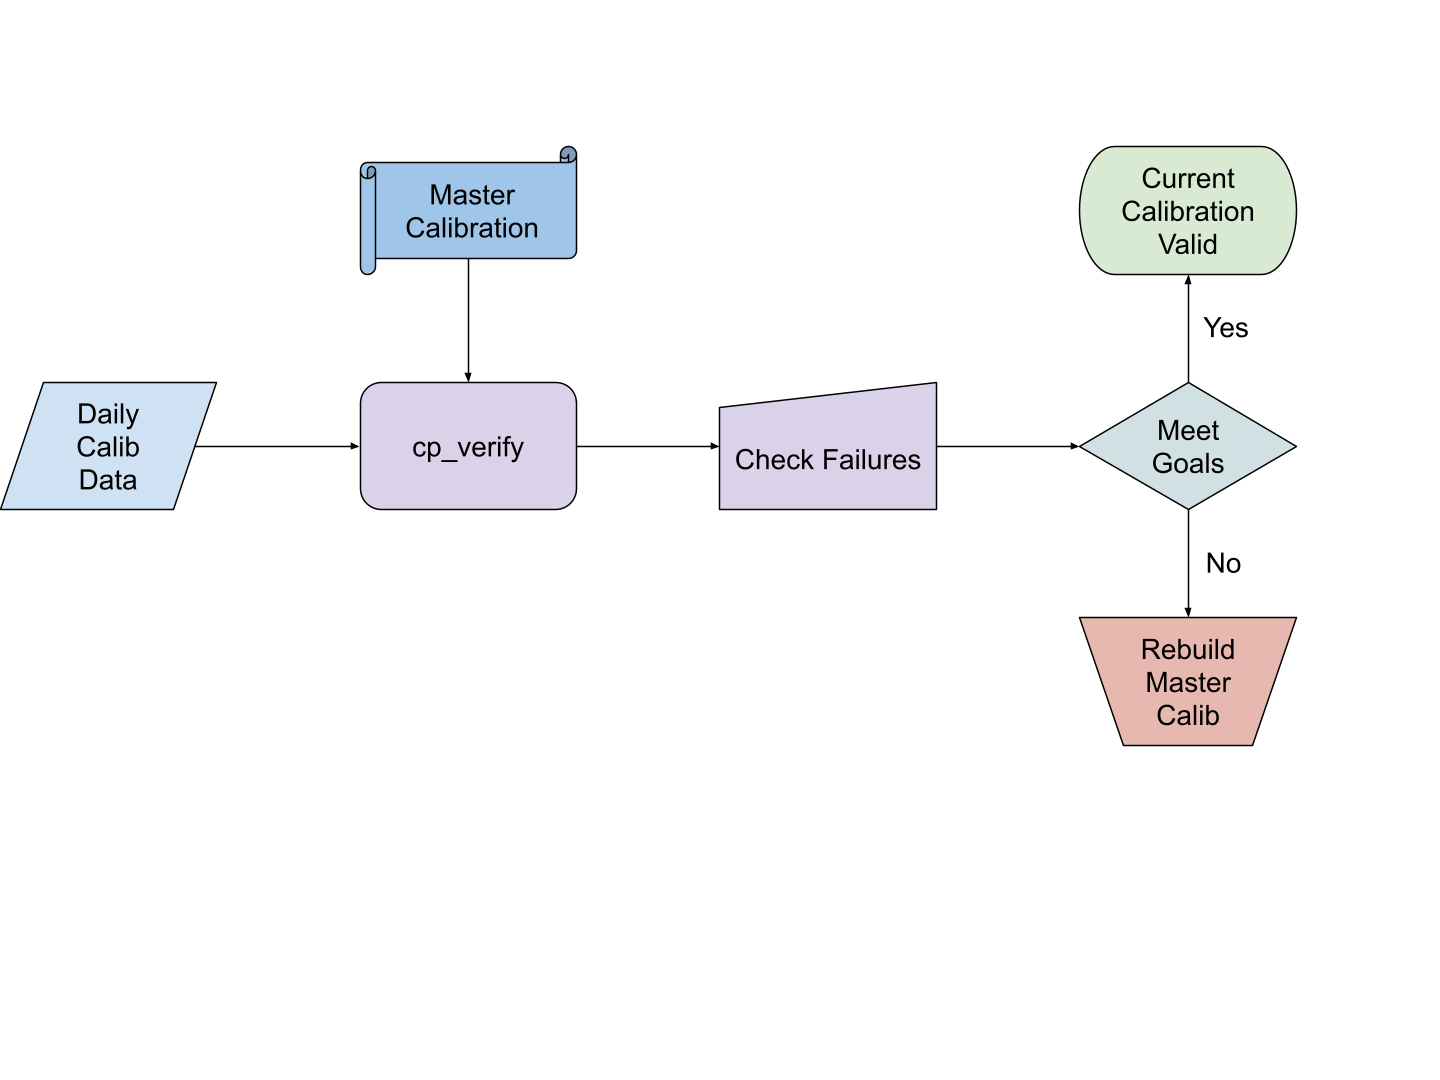
\includegraphics[width=\linewidth]{figures/daily_processing.png}
  \caption{Flowchart of the daily calibration process.}
  \label{fig:daily}
\end{figure}

\section{Curated Calibrations}

Curated calibrations are those calibrations that cannot easily be generated from a series of exposures, or that require special hardware that will not be available at the summit.
Currently, the camera geometry calibration is the most important curated calibration in wide use.
These calibrations are ingested via the \verb|butler write-curated-calibrations| command.
This command by default will attempt to write to the main \verb|$INSTRUMENT/calib| collection.
This is generally not desired, as it is useful for that collection name to point to a CHAINED butler collection, to allow for the calibration management process described above.
Instead, a JIRA ticketed collection name should be used, as the following example illustrates for the LATISS camera:
\begin{verbatim}
butler write-curated-calibrations $REPO lsst.obs.lsst.Latiss \
       --collection LATISS/calib/DM-XYZ --label DM-XYZ
\end{verbatim}

This will ensure that the calibrations can be chained into the main collection as detailed above.

\section{Full Calibration Example}

\section{Conclusions}

\appendix
% Include all the relevant bib files.
% https://lsst-texmf.lsst.io/lsstdoc.html#bibliographies
\section{References} \label{sec:bib}
\renewcommand{\refname}{} % Suppress default Bibliography section
\bibliography{local,lsst,lsst-dm,refs_ads,refs,books}

% Make sure lsst-texmf/bin/generateAcronyms.py is in your path
\section{Acronyms} \label{sec:acronyms}
\addtocounter{table}{-1}
\begin{longtable}{p{0.145\textwidth}p{0.8\textwidth}}\hline
\textbf{Acronym} & \textbf{Description}  \\\hline

DM & Data Management \\\hline
DMTN & DM Technical Note \\\hline
LATISS & LSST Atmospheric Transmission Imager and Slitless Spectrograph \\\hline
LOVE & LSST Operations Visualization Environment \\\hline
PTC & Photon Transfer Curve \\\hline
US & United States \\\hline
USDF & United States Data Facility \\\hline
\end{longtable}

% If you want glossary uncomment below -- comment out the two lines above
%\printglossaries





\end{document}
